% 2010 年安徽卷文科第 21 题：圆心在 x 轴正半轴上、与直线 y=(√3/3)x 相切的一列外切圆。
% 来源 PDF：普通高考/2010/2010安徽文.pdf，SHA-256 1bd928e09356787e648fa9efb9b4c1525f26334f65b08ba82fc736ebb110a4cb。
% 原页：第 2 页（A3 三栏）第 3 栏中部，书页码 572。
% 重绘依据：r_{n+1}=3r_n，圆心横坐标 x_n=2r_n；图中按 r1=1 的比例画出前三个圆
%   （半径 1、3、9，按 0.18 缩放），三圆依次外切且均与直线相切。
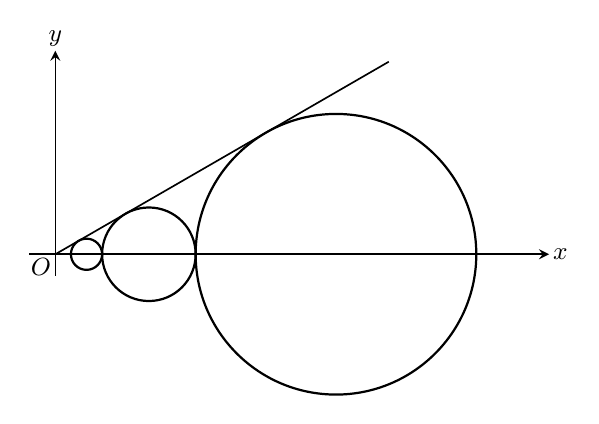
\begin{tikzpicture}[semithick, scale=1.1, every node/.style={inner sep=1.2pt, font=\small}]
  \draw[-stealth] (-0.3,0) -- (5.7,0) node[right] {$x$};
  \draw[-stealth] (0,-0.25) -- (0,2.35) node[above] {$y$};
  \draw (0,0) -- (3.85,2.223);
  \draw[thick] (0.36,0) circle (0.18);
  \draw[thick] (1.08,0) circle (0.54);
  \draw[thick] (3.24,0) circle (1.62);
  \node[below left] at (0,0) {$O$};
\end{tikzpicture}
